%\documentclass[sigconf, authordraft]{acmart}
\documentclass[sigconf]{acmart}

\usepackage{booktabs} % For formal tables

\usepackage{caption}
\usepackage{subcaption}
\usepackage{algorithm}
\usepackage{algpseudocode}
\usepackage[utf8]{inputenc}


% Copyright
%\setcopyright{none}
%\setcopyright{acmcopyright}
%\setcopyright{acmlicensed}
\setcopyright{rightsretained}
%\setcopyright{usgov}
%\setcopyright{usgovmixed}
%\setcopyright{cagov}
%\setcopyright{cagovmixed}


% DOI
\acmDOI{10.1145/nnnnnnn.nnnnnnn}

% ISBN
\acmISBN{978-x-xxxx-xxxx-x/YY/MM}

% Conference
\acmConference[GECCO '19]{the Genetic and Evolutionary Computation Conference 2019}{July 13--17, 2019}{Prague, Czech Republic}
\acmYear{2019}
\copyrightyear{2019}

%\acmArticle{4}
\acmPrice{15.00}

\author{Samuel N. Richter}
\affiliation{
	\institution{Missouri University of Science and Technology \\ Natural Computation Lab}
	\city{Rolla} 
	\state{Missouri} 
	\country{U. S. A.}
}
\email{snr359@mst.edu}

\author{Michael G. Schoen}
\affiliation{
	\institution{Missouri University of Science and Technology \\ Natural Computation Lab}
	\city{Rolla} 
	\state{Missouri} 
	\country{U. S. A.}
}
\email{ms778@mst.edu}

\author{Daniel R. Tauritz}
\affiliation{
	\institution{Missouri University of Science and Technology \\ Natural Computation Lab}
	\city{Rolla} 
	\state{Missouri} 
	\country{U. S. A.}
}
\email{dtauritz@acm.org}

% These commands are optional
%\acmBooktitle{Transactions of the ACM Woodstock conference}
%\editor{Jennifer B. Sartor}
%\editor{Theo D'Hondt}
%\editor{Wolfgang De Meuter}


\begin{document}
\title[Evolving Mean-Update Selection Methods for CMA-ES]{Evolving Mean-Update Selection Methods for CMA-ES}


%
% The code below should be generated by the tool at
% http://dl.acm.org/ccs.cfm
% Please copy and paste the code instead of the example below. 
%
\begin{abstract}
The CMA-ES algorithm searches a fitness landscape by sampling from a multivariate normal distribution and updating its mean by taking a weighted average of the highest fitness candidate solutions. In this work, we explore the possibility of using Genetic Programming to evolve new mean-update selection methods that take into account information other than just raw fitness values. These results may show that CMA-ES can be tuned to specific problem classes to achieve better results.
\end{abstract}

\begin{CCSXML}
	<ccs2012>
	<concept>
	<concept_id>10010147.10010257.10010293.10011809.10011813</concept_id>
	<concept_desc>Computing methodologies~Genetic programming</concept_desc>
	<concept_significance>500</concept_significance>
	</concept>
	<concept>
	<concept_id>10003752.10003809</concept_id>
	<concept_desc>Theory of computation~Design and analysis of algorithms</concept_desc>
	<concept_significance>300</concept_significance>
	</concept>
	<concept>
	<concept_id>10011007.10011074.10011092.10011782.10011813</concept_id>
	<concept_desc>Software and its engineering~Genetic programming</concept_desc>
	<concept_significance>300</concept_significance>
	</concept>
	</ccs2012>
\end{CCSXML}

\ccsdesc[500]{Computing methodologies~Genetic programming}
\ccsdesc[300]{Theory of computation~Design and analysis of algorithms}
\ccsdesc[300]{Software and its engineering~Genetic programming}

\keywords{Selection, Genetic Programming, Hyper-heuristic, CMA-ES}


\maketitle



% ... introduction chapter ...
\section{Introduction}
\label{Introduction}

EAs employ selection functions to control the method by which an individual's genes are selected, for purposes such as, recombination, survival, or updating internal variables. Each selection algorithm plays a significant role in determining the behavior of the EA and the population, and thus, the average performance of the EA's search through the space of solutions~\citep{woodward2010metaBias}.

New selection algorithms can be designed in cases where the performance offered by existing algorithms is insufficient, even with well-tuned parameters. However, the full space of selection algorithms is only limited by the maximum algorithm size, and so it is highly unlikely that any conventionally human-designed algorithm offers the optimal selection behavior, given a specific problem. A performance gain is likely to be attained by exploring the space of selection algorithms to find one that offers better performance than any conventional selection algorithm. Previous work has confirmed this hypothesis, prompting our approach to use a hyper-heuristic, with both generative and perturbative elements, to explore the space of new selection functions ~\citep{woodward2011selection}.


\section{Encoding Selection Functions}
\label{Encoding Selection Functions}

We developed a generalized format to represent a selection function, which can encode both a number of traditional selection functions as well as novel selection functions. The representation consists of two major parts. The first part is a binary Koza-style GP-Tree~\citep{koza1994genetic}. Tthe GP-Tree encodes a mathematical function. All of the function inputs (the terminals of the GP-Tree) are real-valued numbers, and all of the operators in the GP-Tree operate on, and return, real-valued numbers. The terminals of the GP-Tree include various factors pertinent to a single individual of the population, including the individual's fitness, the individual's fitness ranking among the population members, the euclidean distance to the average genome, and the individual's age, in generations. The possible terminal inputs also include information pertinent to the evolution at large, including the total size of the population, the current generation, the maximum and minimum fitness values in the population, and the sum of the individuals' fitness values. Constants are also included, as well as random terminals, which return a random number within a (configurable) closed range. Binary operators in the GP-Tree include various arithmetic and other mathematic functions. When evaluated, the mathematical function encoded by the GP-Tree returns a single real-valued number, corresponding to the relative ``desirability'' of the individual whose data was input into the function. This GP-Tree is built by the generative part of the hyper-heuristic, and can encompass any valid parse tree built from the available operators and terminals.

The second part of the evolved selection function is a method of selecting individuals based on their desirabilities, as calculated by the mathematical function encoded by the GP-Tree. The possible selection methods are inspired by traditional selection functions, such as truncation, tournament selection, fitness-proportional selection, and stochastic universal sampling. Some selection methods will select with replacement, allowing a single individual to be selected more than once per generation. This component is the part of the selection function built by the perturbative hyper-heuristic, being exactly one choice from a set of pre-determined methods.

To perform selection on a population, the function encoded by the GP-Tree is evaluated once for each member of the population, using the data points for that individual (fitness value, fitness ranking, etc.) as inputs to the function. The number output by the function becomes the desirability score for each individual. Finally, the selection step is used to select individuals based on the individuals' desirability scores. The selected individuals can then be used for recombination, as the survivors for the next generation, or for any other update to the internal variables that depends on a chosen subset of the population, as pertinent to the evolutionary search strategy used.


\begin{figure}
	\centering
	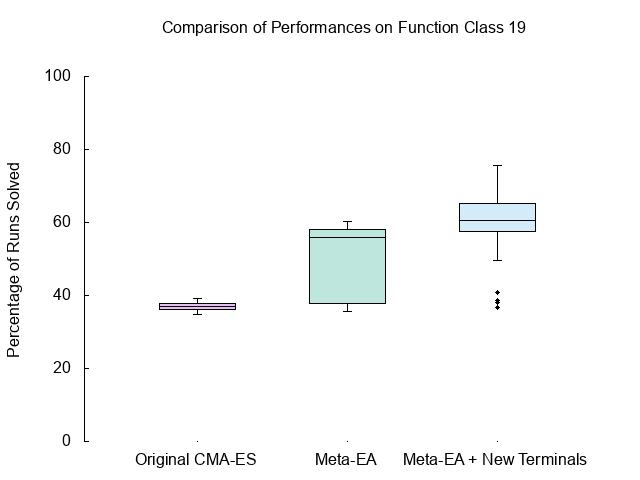
\includegraphics[width=0.45\textwidth]{terminalPerformanceComp}
	\caption{Comparing CMA-ES performance for base, meta-EA evolved, and expanded terminal meta-EA evolved cases.}
	\label{fig:terminalPerformanceComp}
\end{figure}

\section{Search Methodology}
\label{Search Methodology}

We use a meta-EA to develop the selection functions, treating each complete selection function as a member of a higher-order population. After generating an initial pool of randomly constructed selection functions, the quality of each complete selection function is determined, and well-performing selection functions are chosen to recombine and mutate into new candidate selection functions. The size of the trees is constrained using parsimony pressure.

To test our methodology, we target the CMA-ES algorithm for improvement, evolving a new selection function for the mean-update algorithm.

The quality of each selection function is determined by running CMA-ES on a suite of static training instances from a benchmark problem class. The benchmark problem classes used for the underlying EA are selected from the Comparing Continuous Optimizers (COCO) platform used for the GECCO Workshops on Real-Parameter Black-Box Optimization Benchmarking~\citep{cocobbob}. The COCO platform provides 24 unique benchmark problems. Each problem is offered in multiple dimensions, and for each dimension, multiple problem instances are present. We select 11 of the 24 problem classes, and use dimensions 2, 3, 5, and 10. For each class and dimension, we use some instances for the meta-EA, and set aside the rest of the instances to test for generalization. The problem classes were selected by running unodified CMA-S on each of the 24 problem classes, selecting those where it failed to solve some dimension $D \leq 10$ on at least half of the trial runs.

After the initial results were obtained, the authors wanted to investigate the effects that different terminals had on the performance of the modified CMA-ES. Additional terminals tested were genome's Euclidean distance to the best genome found during the run, generations since the last improvement in fitness, and last generations average fitness. The effects of adding and removing terminals were on function classes 3, 16, 19, and 21 with dimension set to 2. These function classes were chosen with no particular bias other than picking function classes where both the modified CMA-ES did not reach a 100 percent success rate. Different sets of terminals were tested by hand until the authors found significant results. The performance of these terminal sets was compared by averaging the ending performance of the modified CMA-ES over 30 runs for each terminal set.


\section{Results and Discussion}
\label{Results}

For the function classes 4 and 19, the success rate of CMA-ES increased by 20-30 percent when modified with the evolved selection function at $D=2$, but performed similarly to the unmodified CMA-ES at other dimensionalities. For function classes 20 and 21, a performance increase is seen on dimensionalities $D=2, 3,$ and $5$, but not $D=10$; curiously, the modified CMA-ES performs worse on function class 21 when $D=10$. For function classes 6 and 12, performance is similar for $D=2, 3,$ and $5$, but for $D=10$, there is a significant performance increase: on function 6, the success rate increased from 0 percent to around 96 percent, and on function class 12, the success rate increased from 18-67 percent, varying across the function instances, to 100 percent for all function instances.

For the function classes 3, 15, 16, 23, and 24, there was no major difference between the success rate of the modified and unmodified CMA-ES.

We observed that evolving a new selection function for CMA-ES increased its solution quality on 6 of the 11 functions tested. In particular, we observed two cases with high dramatic improvements: the tests for COCO function classes 6 and 12 for dimensionality $D=10$. In the case of function class 6, the unmodified CMA-ES was unable to solve any of the testing instances, but the CMA-ES using the evolved selection solved these instances nearly 100\% of the time. In the case of function class 12, the success rate of the unmodified CMA-ES varied strongly between instances, ranging from 18 to 67\%, with an average success rate of 44.05\% across all instances. The modified CMA-ES, however, solved every test instance, reaching the global best fitness in each of 200 runs, on each of the testing instances, achieving a 100\% success rate. By observing the increases in success rate for some of the functions, it is clear that evolving a new selection scheme for CMA-ES provides a substantial benefit in some cases. 

The five cases where no improvement was observed involved functions that were highly multimodal. Three of these function were variants of the Rastrigin function, a highly multimodal function and the other two---the Weierstrass Function and the Katsuura Function---are highly rugged. It is likely, in these cases, that CMA-ES requires some other improvement aside from a new selection scheme to better learn and traverse the global structures of these functions. Because we only replaced the selection scheme of CMA-ES, we only changed how it internally updates the mean. Improving the performance of CMA-ES on these functions likely requires more intelligent updating of the other internal variables of CMA-ES, such as the evolution paths, the covariance matrix, and the step size.

$F=21$, $D=10$ is the one case tested where CMA-ES performed markedly worse than unmodified CMA-ES. This effect is likely due to overspecialization to the set of training instances.

In the investigiation of the effects of changing the terminal set, only one additional terminal was found to have a significant effect on the performance of the modified CMA-ES: Euclidean distance to best-found genome during the entire run. This significant boost in performance was seen only if Euclidean distance to the average genome was also included in the terminal set. Function class 3's success rate went from 32.09\% to 58.51\%, function class 16's from 65.57\% to 68.91\%, function class 19's from 50.21\% to 59.20\%, and function class 23's from 71.56\% to 86.07\%. These results are summarized in Figure~\ref{fig:terminalPerformanceComp}

The benefit of the additional terminals is clear from the four function classes tested. The fact that the two Euclidean distance terminals only boost performance significantly when together, and barely at all if one or both are removed, suggests that these two terminals are working together to provide the boost in performance. It is likely that outliers shown in Figure~\ref{fig:terminalPerformanceComp} are caused by this relationship between these two terminals not forming. These results suggest that further investigation into new terminals could lead to significant improvements in the modified-CMAE-ES's performance.

\section{Conclusions}
\label{Conclusion}
We hypothesized that a hyper-heuristic search through the space of selection functions for EAs could improve the performance of an EA on a particular problem class by discovering a specialized selection function. We developed a representation of selection functions that uses a Koza-style GP-Tree to relate an individual's fitness value and fitness ranking to its relative probability of selection, and used a meta-EA to search through the space of selection functions in this representation. 

With this meta-EA, we have shown that it is possible to generate new selection functions, tuned to a particular benchmark problem, that can enable an EA to significantly outperform conventional selection functions on those problems. Thus, we show that, in order to discover the optimum selection method for an EA operating on a particular problem, it may not be sufficient to use any of the static conventional selection functions tested. We have also shown that, in some cases, this performance increase from a custom selection algorithm will generalize to similar problems in the same problem class. Therefore, if one expects to run the same EA on many problems from the same problem class, one might expect to gain a performance increase by doing some \textit{a priori} calculation to develop a specialized selection algorithm trained on instances of that problem class, which would then enable an EA utilizing that selection function to perform better on other instances of that problem class. However, our experiments have also shown that, for certain functions, replacing only the selection function may not yield significant performance improvements, depending on the behavior of the search strategy and the nature of the function being optimized by the EA. Careful consideration must be given to determine what the effect of tuning the selection scheme of a given EA will be on the performance of that EA, and whether such tuning will cause the EA to have an appreciable performance increase on the problem class in question. 


\end{document}
